\documentclass[a4paper,14pt]{extarticle} % Используем extarticle для поддержки шрифта 14
\usepackage[utf8]{inputenc}
\usepackage[T2A]{fontenc}
\usepackage[russian]{babel}
\usepackage{amsmath}
\usepackage{amssymb}
\usepackage{graphicx}
\usepackage[left=3cm,right=2cm,top=2cm,bottom=2cm]{geometry}
\linespread{1.5}

\begin{document}

\begin{titlepage}
    \begin{center}
        \large
        Министерство науки и высшего образования Российской Федерации \\
        Санкт-Петербургский государственный электротехнический университет \\
        \textbf{«ЛЭТИ» им. В.И. Ульянова (Ленина)} \\
        Кафедра систем автоматического управления

        \vfill

        \textbf{Курсовая работа} \\
        по дисциплине \\
        \textbf{«Электроприводные системы подвижных объектов»}

        \vfill

        Студент группы 9492 \hfill Викторов А.Д. \\
        Преподаватель \hfill Гаврилов С.В.

        \vfill
        Санкт-Петербург \\
        2024
    \end{center}
\end{titlepage}

\setcounter{page}{2}

\newpage

\section*{Введение}

Синхронные двигатели с постоянными магнитами (СДПМ) востребованы в различных областях индустрии и бытовых приложений благодаря своей высокой энергоэффективности, компактности и надёжности. Они находят применение в таких сферах, как промышленное оборудование, системы автоматизации, транспорт, бытовая техника и альтернативная энергетика. Особенности конструкции, включающие использование постоянных магнитов на роторе, позволяют значительно снизить потери энергии, повысить плотность мощности и улучшить эксплуатационные характеристики.

В современных условиях возрастающего спроса на энергоэффективные решения, СДПМ играют ключевую роль в обеспечении экологически чистых технологий. Это обусловливает необходимость разработки и совершенствования систем управления, способных обеспечивать высокую точность регулирования, минимизацию энергопотребления и надежную эксплуатацию оборудования.

Данная курсовая работа посвящена разработке и настройке системы управления для электропривода с синхронным двигателем на постоянных магнитах. В рамках исследования рассматриваются теоретические основы работы таких двигателей, выбираются оптимальные методы управления и моделируются алгоритмы для достижения максимальной эффективности работы системы.

\section*{Постановка задачи}

\begin{enumerate}
\item Исследование теоретических основ работы синхронного двигателя с постоянными магнитами.
\item Выбор архитектуры системы управления.
\item Моделирование и проверка алгоритмов управления.
\item Реализация системы в области программно-аппаратной части.
\end{enumerate}

\section*{Теоретическая часть}

\subsection*{Принцип работы СДПМ}

Синхронные двигатели с постоянными магнитами (СДПМ) включают ротор, основанный на постоянных магнитах, и статор, содержащий обмотки, в которых генерируется магнитное поле. Основной принцип работы этих двигателей заключается во взаимодействии магнитного поля ротора с вращающимся полем статора, что приводит к созданию крутящего момента и вращению ротора с синхронной скоростью.

\subsubsection*{Уравнения электромагнитных процессов}

Основные уравнения, описывающие работу СДПМ, можно выразить следующим образом:

Уравнения напряжений в обмотках статора:
\begin{equation}
\begin{aligned}
u_d &= R_s i_d + \frac{d\psi_d}{dt} - \omega \psi_q, \
u_q &= R_s i_q + \frac{d\psi_q}{dt} + \omega \psi_d,
\end{aligned}
\end{equation}
где $u_d$, $u_q$ — составляющие напряжения в $d$- и $q$-осях; $R_s$ — сопротивление обмоток статора; $i_d$, $i_q$ — составляющие тока в $d$- и $q$-осях; $\psi_d$, $\psi_q$ — потокосцепления; $\omega$ — угловая скорость вращения.

Уравнения потокосцеплений:
\begin{equation}
\begin{aligned}
\psi_d &= L_d i_d + \psi_m, \
\psi_q &= L_q i_q,
\end{aligned}
\end{equation}
где $L_d$, $L_q$ — индуктивности в $d$- и $q$-осях; $\psi_m$ — потокосцепление от постоянных магнитов.

Электромагнитный момент:
\begin{equation}
T_e = \frac{3}{2} p \left(\psi_d i_q - \psi_q i_d\right),
\end{equation}
где $T_e$ — электромагнитный момент; $p$ — число пар полюсов.

Механическое уравнение движения ротора:
\begin{equation}
J\frac{d\omega}{dt} = T_e - T_L - B\omega,
\end{equation}
где $J$ — момент инерции ротора; $T_L$ — нагрузочный момент; $B$ — коэффициент вязкого трения.

\subsubsection*{Пояснение к уравнениям}

Уравнения напряжений описывают динамику токов в обмотках статора в зависимости от приложенного напряжения и параметров двигателя. Уравнения потокосцеплений связывают токи с магнитным потоком, включая вклад постоянных магнитов на роторе. Уравнение электромагнитного момента показывает, как взаимодействие токов и потокосцеплений формирует вращающий момент. Механическое уравнение описывает движение ротора под воздействием моментов.

Эти уравнения являются основой для разработки систем управления, таких как векторное управление и управление с ориентацией на поле (FOC).

\begin{figure}[h]
    \centering
    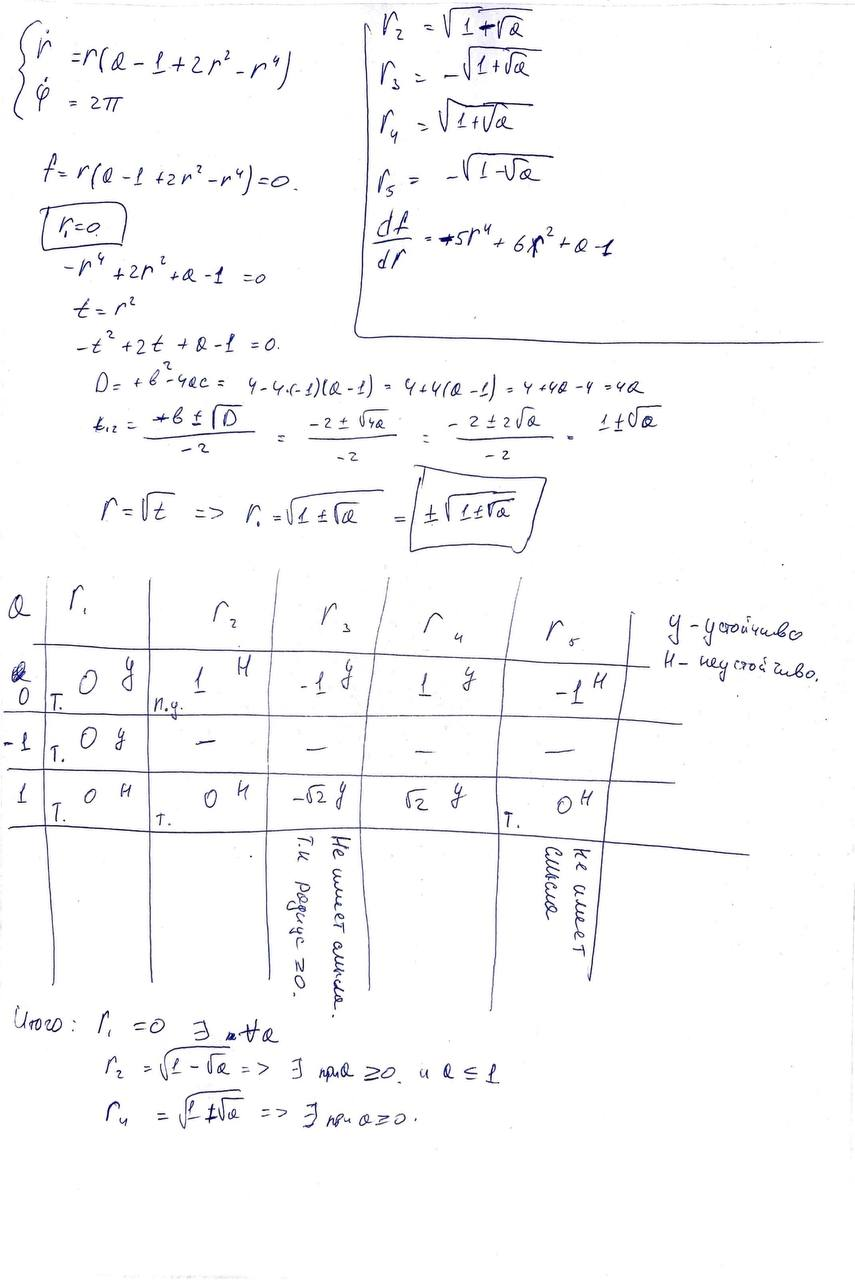
\includegraphics[width=0.8\linewidth]{1.jpg}
    \caption{Структура статора и ротора СДПМ}
    \label{fig:mpr}
\end{figure}

Также важно отметить, что синхронные двигатели с постоянными магнитами обладают высокой точностью и стабильностью работы благодаря отсутствию скольжения, что делает их незаменимыми в системах, требующих высокой точности позиционирования. Включение блока управления позволяет регулировать частоту и амплитуду питающего напряжения для достижения оптимальной работы двигателя.

\subsection*{Преимущества и области применения}

Синхронные двигатели с постоянными магнитами (СДПМ) имеют широкий спектр преимуществ, которые делают их привлекательными для использования в различных отраслях. Одним из основных достоинств является высокая энергоэффективность, достигаемая благодаря минимальным потерям на возбуждение. Конструкция с постоянными магнитами обеспечивает также компактность и высокую плотность мощности, что критически важно в условиях ограниченного пространства.

Особое внимание следует уделить применению СДПМ в области робототехники. В современных робототехнических системах такие двигатели используются для обеспечения прецизионного управления движением, особенно в манипуляторах, автоматических транспортных средствах и других мобильных роботах. Высокая точность работы двигателей позволяет значительно улучшить точность позиционирования, что особенно важно для выполнения сложных операций, таких как сборка, сварка или работа в условиях, где требуется минимальный допуск.

Кроме того, СДПМ находят широкое применение в электромобилях и беспилотных летательных аппаратах, где компактность и энергоэффективность играют ключевую роль. Например, использование таких двигателей позволяет увеличить запас хода транспортных средств за счёт более эффективного использования энергии аккумуляторов. Также в промышленных системах автоматизации СДПМ обеспечивают точное выполнение операций при минимальном энергопотреблении.

\begin{figure}[h]
    \centering
    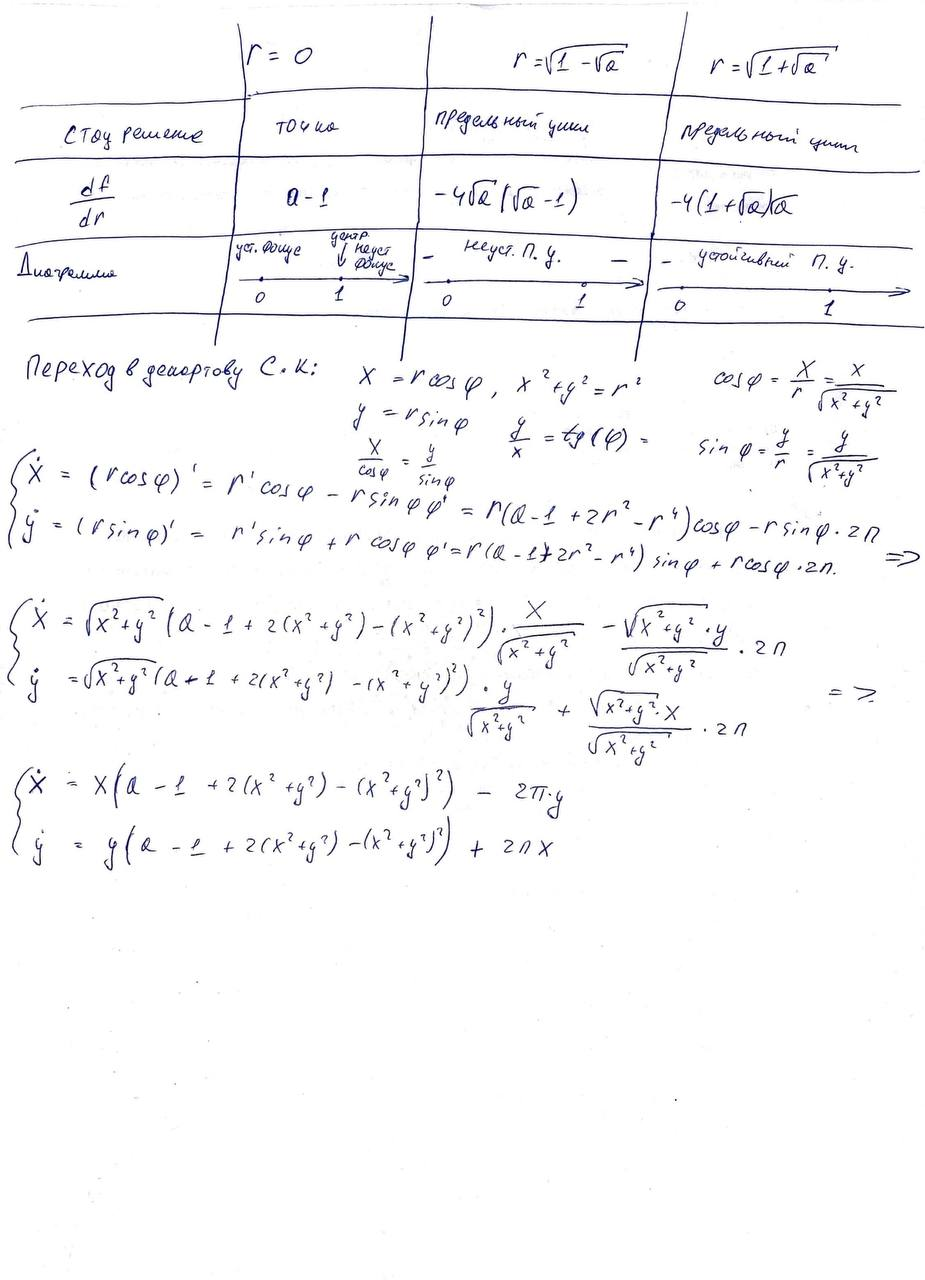
\includegraphics[width=0.8\linewidth]{2.jpg}
    \caption{Применение СДПМ в робототехнике}
    \label{fig:mpr}
\end{figure}

\section*{Разработка системы управления}

\subsection*{Выбор методов управления}

Для управления синхронными двигателями с постоянными магнитами (СДПМ) используется несколько методов, каждый из которых имеет свои особенности и область применения. Ниже представлены основные подходы к управлению:

\subsection*{Скалярное управление}

Скалярное управление, также известное как управление по $U/f$, является наиболее простым методом. В основе лежит поддержание постоянного соотношения между напряжением и частотой питания двигателя, что позволяет управлять скоростью вращения ротора. Этот метод предполагает регулирование входного напряжения и частоты таким образом, чтобы величина магнитного потока в двигателе оставалась постоянной. Преимущества скалярного управления включают простоту реализации и невысокую стоимость. Однако этот метод обладает рядом ограничений, таких как снижение точности управления при низких скоростях.

\subsubsection*{Основные уравнения скалярного управления}

Соотношение между напряжением и частотой:
\begin{equation}
\frac{U}{f} = \text{const},
\end{equation}
где $U$ — амплитуда входного напряжения, $f$ — частота питания двигателя.

Момент двигателя:
\begin{equation}
T_e \propto \frac{U^2}{f^2},
\end{equation}
где $T_e$ — электромагнитный момент двигателя. Это уравнение показывает, что при увеличении частоты необходимо пропорционально увеличивать напряжение, чтобы сохранить стабильный момент.

Уравнение магнитного потока:
\begin{equation}
\psi \propto \frac{U}{f},
\end{equation}
где $\psi$ — потокосцепление. Для поддержания оптимального магнитного потока важно сохранять соотношение $U/f$ неизменным.

\subsubsection*{Алгоритм реализации}

Скалярное управление обычно реализуется следующим образом:
\begin{enumerate}
\item Определяется требуемая скорость вращения ротора.
\item Рассчитывается соответствующая частота питания двигателя.
\item Вычисляется необходимое напряжение с учётом постоянного соотношения $U/f$.
\item Формируется сигнал для инвертора, который обеспечивает подачу рассчитанных напряжения и частоты.
\end{enumerate}

\subsubsection*{Преимущества и недостатки}

Преимущества скалярного управления:
\begin{itemize}
\item Простота реализации.
\item Низкая стоимость оборудования.
\item Подходит для приложений с невысокими требованиями к точности управления.
\end{itemize}

Недостатки:
\begin{itemize}
\item Снижение эффективности при низких скоростях.
\item Ограниченные возможности динамического управления.
\item Необходимость использования внешних датчиков для компенсации нестабильности.
\end{itemize}

Скалярное управление часто используется в системах, где требования к точности невысоки, например, в насосах, вентиляторах и других установках с постоянной нагрузкой. Однако в системах, требующих высокой точности и быстродействия, предпочтение отдают более сложным методам, таким как векторное управление или управление с ориентацией на поле (FOC).


\subsection*{Векторное управление}

Векторное управление (Field-Oriented Control, FOC) является одним из самых популярных и эффективных методов управления синхронными двигателями с постоянными магнитами. Этот подход позволяет управлять электромагнитным моментом двигателя независимо от магнитного потока, что обеспечивает высокую точность и динамичность системы.

\subsubsection*{Принципы работы векторного управления}

Основная идея векторного управления заключается в преобразовании трёхфазной системы координат статора в двухфазную систему координат $dq$, которая вращается синхронно с магнитным полем ротора. Это позволяет разделить токи статора на две компоненты:
\begin{itemize}
\item $i_d$ — составляющая тока, ответственная за создание магнитного потока.
\item $i_q$ — составляющая тока, отвечающая за создание электромагнитного момента.
\end{itemize}

\subsubsection*{Основные уравнения векторного управления}

Уравнения преобразования в систему координат $dq$:
\begin{equation}
i_d = \frac{2}{3} \left( i_a - \frac{1}{2}i_b - \frac{1}{2}i_c \right),
\end{equation}
\begin{equation}
i_q = \frac{2}{3} \left( 0 + \frac{\sqrt{3}}{2}i_b - \frac{\sqrt{3}}{2}i_c \right),
\end{equation}
где $i_a$, $i_b$, $i_c$ — токи фаз статора.

Электромагнитный момент двигателя:
\begin{equation}
T_e = \frac{3}{2}p\psi i_q,
\end{equation}
где $p$ — число пар полюсов, $\psi$ — потокосцепление ротора.

Управляющие напряжения в системе координат $dq$:
\begin{equation}
v_d = R_s i_d - \omega \psi + L_d \frac{di_d}{dt},
\end{equation}
\begin{equation}
v_q = R_s i_q + \omega L_q i_q + L_q \frac{di_q}{dt},
\end{equation}
где $R_s$ — сопротивление обмотки статора, $L_d$, $L_q$ — индуктивности по осям $d$ и $q$, $\omega$ — угловая скорость.

\subsubsection*{Алгоритм реализации}

Измерение токов фаз статора ($i_a$, $i_b$, $i_c$).

Преобразование токов в систему координат $dq$.

Вычисление требуемых значений $i_d$ и $i_q$ в зависимости от заданного момента и потока.

Расчёт управляющих напряжений $v_d$ и $v_q$ с использованием регуляторов ПИД.

Обратное преобразование из координат $dq$ в трёхфазную систему для подачи сигналов на инвертор.

\subsubsection*{Преимущества и недостатки}

Преимущества:
\begin{itemize}
\item Высокая точность управления моментом и скоростью.
\item Хорошая динамическая характеристика.
\item Оптимизация энергопотребления.
\end{itemize}

Недостатки:
\begin{itemize}
\item Сложность реализации.
\item Высокие требования к вычислительным ресурсам контроллера.
\item Необходимость точного определения параметров двигателя.
\end{itemize}

Векторное управление является стандартом для высокоточных и динамичных приложений, таких как робототехника, электромобили и авиационные системы.

\subsection*{Управление с ориентацией на поле (FOC)}

Управление с ориентацией на поле (Field-Oriented Control, FOC) является разновидностью векторного управления, которое обеспечивает независимое регулирование магнитного потока и электромагнитного момента двигателя. Этот метод позволяет достичь высокой точности управления и оптимального использования энергии.

\subsubsection*{Основные уравнения FOC}

Компоненты токов в системе координат $dq$:
\begin{equation}
i_d = \frac{2}{3} \left( i_a - \frac{1}{2}i_b - \frac{1}{2}i_c \right),
\end{equation}
\begin{equation}
i_q = \frac{2}{3} \left( 0 + \frac{\sqrt{3}}{2}i_b - \frac{\sqrt{3}}{2}i_c \right).
\end{equation}

Управление потоком и моментом через токи:
\begin{equation}
\psi_d = L_d i_d + \psi_m,
\end{equation}
\begin{equation}
T_e = \frac{3}{2} p \psi i_q,
\end{equation}
где $\psi_m$ — потокосцепление ротора из-за постоянных магнитов.

Уравнения для расчёта напряжений:
\begin{equation}
v_d = R_s i_d - \omega \psi_q + L_d \frac{di_d}{dt},
\end{equation}
\begin{equation}
v_q = R_s i_q + \omega \psi_d + L_q \frac{di_q}{dt}.
\end{equation}

\subsubsection*{Алгоритм реализации}

Измерение токов фаз статора.

Преобразование токов в систему координат $dq$.

Регулирование компонент $i_d$ и $i_q$


\subsection*{Моделирование системы управления}

На рисунке 3 представлена система управления СДПМ построенная согласно описанным выше алгоритмам управления.

\begin{figure}[h]
    \centering
    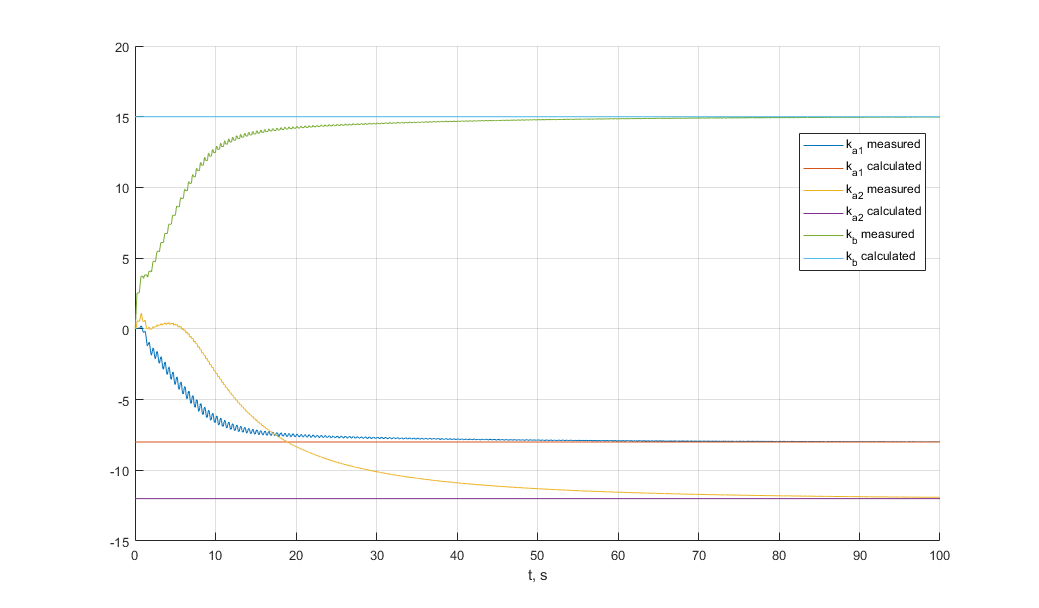
\includegraphics[width=0.8\linewidth]{3.png}
    \caption{Система управления СДПМ}
    \label{fig:mpr}
\end{figure}

На рисунке 4 представлены графики токов СДПМ при моделировании с построенной системой управления.

\begin{figure}[h]
    \centering
    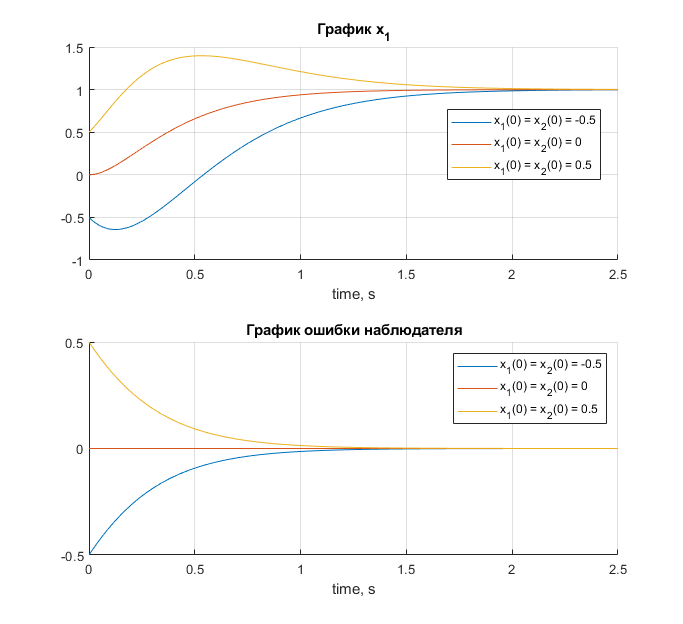
\includegraphics[width=0.8\linewidth]{4.png}
    \caption{График токов фаз СДПМ при моделировании}
    \label{fig:mpr}
\end{figure}

На рисунке 5 представлены графики изменения угла ротора СДПМ и задание на угол поворота при моделировании с построенной системой управления. Само собой не стояло цели подобрать коэффициенты всех регуляторов для того, чтобы двигатель моментально отрабатывал все задания, но проведенное моделирование показывает, что цель - построить систему управления СДПМ достигнута

\begin{figure}[h]
    \centering
    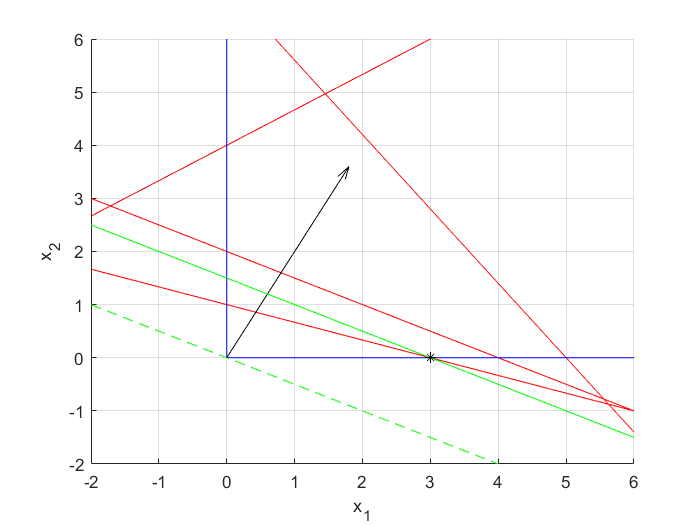
\includegraphics[width=0.8\linewidth]{5.png}
    \caption{График токов фаз СДПМ при моделировании}
    \label{fig:mpr}
\end{figure}

\section*{Выводы}

В ходе выполнения курсовой работы была выполнена разработка системы управления электроприводом с синхронным двигателем с постоянными магнитами (СДПМ). Рассмотрены теоретические основы работы СДПМ, проведён анализ существующих методов управления, а также детально изучены их принципы работы и области применения. На основе проведённого анализа сформированы следующие выводы:

Актуальность использования СДПМ
СДПМ являются одним из наиболее перспективных типов электродвигателей благодаря высокой энергоэффективности, надёжности и компактным размерам. Эти преимущества делают их оптимальным выбором для применения в робототехнике, транспортных системах, промышленных установках и других областях.

Разнообразие методов управления
Рассмотрены три основных метода управления: скалярное управление, векторное управление и управление с ориентацией на поле.

Скалярное управление характеризуется простотой реализации, но ограничено в точности и динамических возможностях.
Векторное управление обеспечивает независимое управление моментом и магнитным потоком, что делает его подходящим для высокоточных приложений.
Управление с ориентацией на поле (FOC) демонстрирует максимальную эффективность благодаря оптимизации работы двигателя при разных нагрузках.
Применение методов управления
Для выбора метода управления необходимо учитывать требования к точности, динамике и эффективности системы. Для робототехники и других высокотехнологичных приложений наиболее предпочтительны методы векторного управления и управления с ориентацией на поле, так как они обеспечивают высокую точность и быстродействие.

Математическое описание работы СДПМ
Разработаны математические модели, описывающие работу двигателя и методы управления. Они позволяют моделировать и оптимизировать процессы управления, что критически важно для сложных приложений, таких как робототехника и автоматизированные системы.

Практическая значимость работы
Результаты данной работы могут быть использованы для разработки систем управления СДПМ в различных областях промышленности и техники. Модели и алгоритмы, рассмотренные в работе, обеспечивают основу для внедрения энергоэффективных и высокоточных решений.

\textbf{Резюмируя}, проведённое исследование подтвердило, что грамотный выбор и настройка методов управления являются ключевыми факторами, обеспечивающими успешное применение СДПМ в современном инженерном мире. Это позволяет достигать высокой эффективности, точности и надёжности электроприводов, что открывает новые горизонты для их использования в самых передовых технологиях.

\end{document}
